\documentclass[letterpaper]{scrartcl}
\usepackage{times}
\usepackage{helvet}
\usepackage{courier}
\usepackage{graphicx}
\usepackage{enumerate}

% for placing figures
\usepackage{float}

% packages for \code command in mydefs
% for code blocks to use Courier New
% \usepackage{fontspec}
% for code block colors
\usepackage[usenames,dvipsnames,svgnames,table]{xcolor}

% for code block writing text in a drawing
\usepackage{tikz}

% for code block syntax highlighting?
\usepackage{listings}

% for fonts in mydefs
\usepackage[style=base,font=small,labelfont=bf]{caption}
\usepackage{subcaption}



\setkomafont{disposition}{\normalfont\bfseries}



\title{Why HUBcheck?}
\subtitle{A case for automated testing of hub components}

\author{
  Derrick S. Kearney \\
  \texttt{dsk@purdue.edu}
}

\date{}



% include my definitions like xcode
%
%  mydefs.tex  2007-03-19  Mark Senn  http://www.ecn.purdue.edu/~mark
%
%  Command definitions that can be used in all documents that have
%      %
%  mydefs.tex  2007-03-19  Mark Senn  http://www.ecn.purdue.edu/~mark
%
%  Command definitions that can be used in all documents that have
%      %
%  mydefs.tex  2007-03-19  Mark Senn  http://www.ecn.purdue.edu/~mark
%
%  Command definitions that can be used in all documents that have
%      \input{mydefs}
%

%%%%%%%%%%%%%%%%%%%%%%%%%%%%%%%%%%%%%%%%%%%%%%%%%%
% setup code single spacing caption for all floats

\captionsetup{
  font={stretch=1},
}

%%%%%%%%%%%%%%%%%%%%%%%%%%%%%%%%%%%%%%%%%%%%%%%%%%


%%%%%%%%%%%%%%%%%%%%%%%%%%%%%%%%%%%%%%%%%%%%%%%%%%
% setup special fonts/format (xformat,xf) for talking about:
%   module
%   classes
%   class methods
%   class attributes (data members)
%   objects
%   locator
%   locator family
%   inline code
%   html link name
%   parameter name
%   uri scheme (http, https, mailto, webdav)
%   program name

\newcommand{\xfmodule}[1]{\texttt{#1}}
\newcommand{\xfclass}[1]{\texttt{#1}}
\newcommand{\xfmethod}[1]{\texttt{#1}}
\newcommand{\xfattribute}[1]{\texttt{#1}}
\newcommand{\xfobject}[1]{\texttt{#1}}
\newcommand{\xflocator}[1]{\texttt{#1}}
\newcommand{\xflocfam}[1]{\texttt{#1}}
\newcommand{\xfinlinecode}[1]{\texttt{#1}}
\newcommand{\xfhtmllink}[1]{\texttt{#1}}
\newcommand{\xfparameter}[1]{\texttt{#1}}
\newcommand{\xfurischeme}[1]{\texttt{#1}}
\newcommand{\xfprogramname}[1]{\textbf{#1}}


%%%%%%%%%%%%%%%%%%%%%%%%%%%%%%%%%%%%%%%%%%%%%%%%%%


%%%%%%%%%%%%%%%%%%%%%%%%%%%%%%%%%%%%%%%%%%%%%%%%%%
% setup code listing captions
%
% i could never figure out why the colorbox seems so indented
% so we just multiply our fboxsep by 7 and that accounts for
% the indentation. had to adjust framexleftmargin and
% framexrightmargin to match.
%

\DeclareCaptionFont{white}{\color{white}}
\DeclareCaptionFormat{listing}{
  \colorbox[cmyk]{0.43, 0.35, 0.35, 0.01}{
    \parbox{\dimexpr\textwidth-7\fboxsep\relax} {
      #1#2#3
    }
  }
}

\captionsetup[lstlisting]{
  format=listing,
  labelfont=white,
  textfont=white,
  singlelinecheck=false,
  margin=0pt,
}

%%%%%%%%%%%%%%%%%%%%%%%%%%%%%%%%%%%%%%%%%%%%%%%%%%


%%%%%%%%%%%%%%%%%%%%%%%%%%%%%%%%%%%%%%%%%%%%%%%%%%
% setting for code listings

\lstset{ %
  basicstyle=\scriptsize\ttfamily,    % the size of the fonts that are used for the code
  breaklines=true,                    % sets automatic line breaking
  captionpos=t,                       % sets the caption-position to bottom
  belowcaptionskip=15px,              % add some space under the caption and above the code
  frame=lines,                        % adds a frame around the code
  numbers=left,                       % where to put the line-numbers; possible values are (none, left, right)
  numbersep=5pt,                      % how far the line-numbers are from the code
  numberstyle=\tiny\color{black},     % the style that is used for the line-numbers
  showspaces=false,                   % show spaces everywhere adding particular underscores;
  showstringspaces=false,             % underline spaces within strings only
  showtabs=false,                     % show tabs within strings adding particular underscores
  stepnumber=1,                       % the step between two line-numbers. If it's 1, each line will be numbered
  stringstyle=\color{black}\ttfamily\textbf, % string literal style
  tabsize=2,                          % sets default tabsize to 2 spaces
  xleftmargin=5ex,                    % space between page margin and line numbers/code/frames
  framexleftmargin=13pt,               % left width of tob/bottom frame, starts at code, excludes line numbers
  framexrightmargin=-3pt,              % right width of top/bottom frame, starts at textwidth?
%  framexbottommargin=5pt,
  extendedchars=true,
  belowskip=15pt,
}

% load languages we will be using
\lstloadlanguages{
  XML,
  HTML,
  Python,
}

\lstnewenvironment{xcode}[1]
  {
    \noindent
    \minipage{\linewidth}
%    \lstset{tabsize=4, belowcaptionskip=1\baselineskip, #1}
    \lstset{tabsize=4, #1}
  }%
  {
    \endminipage
  }

%%%%%%%%%%%%%%%%%%%%%%%%%%%%%%%%%%%%%%%%%%%%%%%%%%

%

%%%%%%%%%%%%%%%%%%%%%%%%%%%%%%%%%%%%%%%%%%%%%%%%%%
% setup code single spacing caption for all floats

\captionsetup{
  font={stretch=1},
}

%%%%%%%%%%%%%%%%%%%%%%%%%%%%%%%%%%%%%%%%%%%%%%%%%%


%%%%%%%%%%%%%%%%%%%%%%%%%%%%%%%%%%%%%%%%%%%%%%%%%%
% setup special fonts/format (xformat,xf) for talking about:
%   module
%   classes
%   class methods
%   class attributes (data members)
%   objects
%   locator
%   locator family
%   inline code
%   html link name
%   parameter name
%   uri scheme (http, https, mailto, webdav)
%   program name

\newcommand{\xfmodule}[1]{\texttt{#1}}
\newcommand{\xfclass}[1]{\texttt{#1}}
\newcommand{\xfmethod}[1]{\texttt{#1}}
\newcommand{\xfattribute}[1]{\texttt{#1}}
\newcommand{\xfobject}[1]{\texttt{#1}}
\newcommand{\xflocator}[1]{\texttt{#1}}
\newcommand{\xflocfam}[1]{\texttt{#1}}
\newcommand{\xfinlinecode}[1]{\texttt{#1}}
\newcommand{\xfhtmllink}[1]{\texttt{#1}}
\newcommand{\xfparameter}[1]{\texttt{#1}}
\newcommand{\xfurischeme}[1]{\texttt{#1}}
\newcommand{\xfprogramname}[1]{\textbf{#1}}


%%%%%%%%%%%%%%%%%%%%%%%%%%%%%%%%%%%%%%%%%%%%%%%%%%


%%%%%%%%%%%%%%%%%%%%%%%%%%%%%%%%%%%%%%%%%%%%%%%%%%
% setup code listing captions
%
% i could never figure out why the colorbox seems so indented
% so we just multiply our fboxsep by 7 and that accounts for
% the indentation. had to adjust framexleftmargin and
% framexrightmargin to match.
%

\DeclareCaptionFont{white}{\color{white}}
\DeclareCaptionFormat{listing}{
  \colorbox[cmyk]{0.43, 0.35, 0.35, 0.01}{
    \parbox{\dimexpr\textwidth-7\fboxsep\relax} {
      #1#2#3
    }
  }
}

\captionsetup[lstlisting]{
  format=listing,
  labelfont=white,
  textfont=white,
  singlelinecheck=false,
  margin=0pt,
}

%%%%%%%%%%%%%%%%%%%%%%%%%%%%%%%%%%%%%%%%%%%%%%%%%%


%%%%%%%%%%%%%%%%%%%%%%%%%%%%%%%%%%%%%%%%%%%%%%%%%%
% setting for code listings

\lstset{ %
  basicstyle=\scriptsize\ttfamily,    % the size of the fonts that are used for the code
  breaklines=true,                    % sets automatic line breaking
  captionpos=t,                       % sets the caption-position to bottom
  belowcaptionskip=15px,              % add some space under the caption and above the code
  frame=lines,                        % adds a frame around the code
  numbers=left,                       % where to put the line-numbers; possible values are (none, left, right)
  numbersep=5pt,                      % how far the line-numbers are from the code
  numberstyle=\tiny\color{black},     % the style that is used for the line-numbers
  showspaces=false,                   % show spaces everywhere adding particular underscores;
  showstringspaces=false,             % underline spaces within strings only
  showtabs=false,                     % show tabs within strings adding particular underscores
  stepnumber=1,                       % the step between two line-numbers. If it's 1, each line will be numbered
  stringstyle=\color{black}\ttfamily\textbf, % string literal style
  tabsize=2,                          % sets default tabsize to 2 spaces
  xleftmargin=5ex,                    % space between page margin and line numbers/code/frames
  framexleftmargin=13pt,               % left width of tob/bottom frame, starts at code, excludes line numbers
  framexrightmargin=-3pt,              % right width of top/bottom frame, starts at textwidth?
%  framexbottommargin=5pt,
  extendedchars=true,
  belowskip=15pt,
}

% load languages we will be using
\lstloadlanguages{
  XML,
  HTML,
  Python,
}

\lstnewenvironment{xcode}[1]
  {
    \noindent
    \minipage{\linewidth}
%    \lstset{tabsize=4, belowcaptionskip=1\baselineskip, #1}
    \lstset{tabsize=4, #1}
  }%
  {
    \endminipage
  }

%%%%%%%%%%%%%%%%%%%%%%%%%%%%%%%%%%%%%%%%%%%%%%%%%%

%

%%%%%%%%%%%%%%%%%%%%%%%%%%%%%%%%%%%%%%%%%%%%%%%%%%
% setup code single spacing caption for all floats

\captionsetup{
  font={stretch=1},
}

%%%%%%%%%%%%%%%%%%%%%%%%%%%%%%%%%%%%%%%%%%%%%%%%%%


%%%%%%%%%%%%%%%%%%%%%%%%%%%%%%%%%%%%%%%%%%%%%%%%%%
% setup special fonts/format (xformat,xf) for talking about:
%   module
%   classes
%   class methods
%   class attributes (data members)
%   objects
%   locator
%   locator family
%   inline code
%   html link name
%   parameter name
%   uri scheme (http, https, mailto, webdav)
%   program name

\newcommand{\xfmodule}[1]{\texttt{#1}}
\newcommand{\xfclass}[1]{\texttt{#1}}
\newcommand{\xfmethod}[1]{\texttt{#1}}
\newcommand{\xfattribute}[1]{\texttt{#1}}
\newcommand{\xfobject}[1]{\texttt{#1}}
\newcommand{\xflocator}[1]{\texttt{#1}}
\newcommand{\xflocfam}[1]{\texttt{#1}}
\newcommand{\xfinlinecode}[1]{\texttt{#1}}
\newcommand{\xfhtmllink}[1]{\texttt{#1}}
\newcommand{\xfparameter}[1]{\texttt{#1}}
\newcommand{\xfurischeme}[1]{\texttt{#1}}
\newcommand{\xfprogramname}[1]{\textbf{#1}}


%%%%%%%%%%%%%%%%%%%%%%%%%%%%%%%%%%%%%%%%%%%%%%%%%%


%%%%%%%%%%%%%%%%%%%%%%%%%%%%%%%%%%%%%%%%%%%%%%%%%%
% setup code listing captions
%
% i could never figure out why the colorbox seems so indented
% so we just multiply our fboxsep by 7 and that accounts for
% the indentation. had to adjust framexleftmargin and
% framexrightmargin to match.
%

\DeclareCaptionFont{white}{\color{white}}
\DeclareCaptionFormat{listing}{
  \colorbox[cmyk]{0.43, 0.35, 0.35, 0.01}{
    \parbox{\dimexpr\textwidth-7\fboxsep\relax} {
      #1#2#3
    }
  }
}

\captionsetup[lstlisting]{
  format=listing,
  labelfont=white,
  textfont=white,
  singlelinecheck=false,
  margin=0pt,
}

%%%%%%%%%%%%%%%%%%%%%%%%%%%%%%%%%%%%%%%%%%%%%%%%%%


%%%%%%%%%%%%%%%%%%%%%%%%%%%%%%%%%%%%%%%%%%%%%%%%%%
% setting for code listings

\lstset{ %
  basicstyle=\scriptsize\ttfamily,    % the size of the fonts that are used for the code
  breaklines=true,                    % sets automatic line breaking
  captionpos=t,                       % sets the caption-position to bottom
  belowcaptionskip=15px,              % add some space under the caption and above the code
  frame=lines,                        % adds a frame around the code
  numbers=left,                       % where to put the line-numbers; possible values are (none, left, right)
  numbersep=5pt,                      % how far the line-numbers are from the code
  numberstyle=\tiny\color{black},     % the style that is used for the line-numbers
  showspaces=false,                   % show spaces everywhere adding particular underscores;
  showstringspaces=false,             % underline spaces within strings only
  showtabs=false,                     % show tabs within strings adding particular underscores
  stepnumber=1,                       % the step between two line-numbers. If it's 1, each line will be numbered
  stringstyle=\color{black}\ttfamily\textbf, % string literal style
  tabsize=2,                          % sets default tabsize to 2 spaces
  xleftmargin=5ex,                    % space between page margin and line numbers/code/frames
  framexleftmargin=13pt,               % left width of tob/bottom frame, starts at code, excludes line numbers
  framexrightmargin=-3pt,              % right width of top/bottom frame, starts at textwidth?
%  framexbottommargin=5pt,
  extendedchars=true,
  belowskip=15pt,
}

% load languages we will be using
\lstloadlanguages{
  XML,
  HTML,
  Python,
}

\lstnewenvironment{xcode}[1]
  {
    \noindent
    \minipage{\linewidth}
%    \lstset{tabsize=4, belowcaptionskip=1\baselineskip, #1}
    \lstset{tabsize=4, #1}
  }%
  {
    \endminipage
  }

%%%%%%%%%%%%%%%%%%%%%%%%%%%%%%%%%%%%%%%%%%%%%%%%%%




\begin{document}
\maketitle

\begin{abstract}
\end{abstract}

\section{Origins of hub testing}

In 2005, the Purdue HUBzero Team supported their first hub,
nanoHUB.org. In 2007, the number of hubs had risen to four, and by 2012, the
team was supporting twenty five hubs. The release of the open source version
allowed others to begin launching self supported hubs.  Each deployed hub
started from a single core version of the software and quickly bloomed into its
own system with the standard set of hub components and slightly different
configurations and content.

Despite the best intentions of the Purdue HUBzero Team, hub software
was, and still is, being released with bugs. The same economies of scale that
allow the group to rapidly deploy quality software, work against the group when
combating erroneous software. A single bug that is discovered on one hub
website is usually also on numerous other hub websites. Different upgrade
schedules of the hubs and a lack of upgrade documentation make it hard to tell
which hubs still have one of the known bugs. The lack of a test suite for
components makes it difficult to find bugs before and after the software is
released.

The testing of hub components is performed by hand and is a time consuming,
error prone process.  Manual testing promotes variation in tests performed. Due
to its repetitive nature, each iteration of testing can be performed a
different way, or not performed, if forgotten. It also promotes spot checking
of fixes to bugs instead of a broad retesting of components due to the elevated
time commitment needed to setup and perform tests.

\section{Related work}
\label{sec:related_work}

Automated tools exist to aid in the testing of web applications and cover the
popular testing topics including performance, security, functionality,
usability, and interface.

One popular class of automated web testing tools are \textit{web crawlers},
like Crawljax and IBM Security AppScan. Web crawlers wonder through a web
application, performing tests based on the existence of interactive widgets
(text boxes, links, and buttons) on web pages.

%For some tools in this class, a
%side effect of web crawling is the creation of a graph with nodes that
%represent the states of the web application and edges that represent the
%actions performed to get to the next state. The paths of the web application
%graph can be analyzed to generate additional tests to be performed.

Web crawlers require very little coordination from the hub developer. Their
meandering nature allows them to treat the web application like a black box
when checking for bugs, reviewing the available widgets on a web page,
attempting actions, and documenting results. This makes them an ideal
application for building site maps, testing navigation, checking for bad links,
and performing security scans across generic web pages. Web crawlers take a
long time to run because their goal is to exhaust every path through a graph
that represents the web application under test.  The upside is that they have
the opportunity to run lots of tests on the web application, in an automated
fashion, with little initial investment of time from developers.

Web crawlers treat the web application like a black box. Knowledge of how the
web application works and its limits are discovered at runtime, which can
require a time consuming, exhaustive searching of the problem space. Even after
the web application has been ``learned'', there is no authority to determine if
the learned behavior is the correct behavior. For example, an important part of
building a successful hub is allowing content developers to develop and deploy
their own resources.  The first step of contributing a resource to the hub is to
fill out a web form describing the content that is being contributed. The
form generally contains text boxes and drop down lists, some of which are
required or have special restrictions on accepted values. A web crawler would
be able to interact with the widgets in the web form, test navigation of links
on the page, and test security of inputting values into the text boxes in the
form.  Without additional knowledge, provided by the developer, the web crawler
would have a hard time determining if a widget was supposed to be required or
optional, or confirming that each widget's input validation was working
properly.
%
%Some web crawlers accumulate history, giving them an advantage during repeated
%runs of the crawler.  Web crawlers that operate without memory need to relearn
%the web application with each run of the crawler, which can be timely when
%testing specific features.
%
% need to cite which web crawlers acculate history that can be fed back into
% the crawler. maybe crawljax probably some of the non testing related
% crawlers.
%
Exploring every path through the web application graph is good for whole system
testing, but when it comes to targeted testing of a specific set of actions,
another class of tools is available.


A second class of automated web testing tools are \textit{test recorders},
including Selenium WebDriver, Webking, and Sahi. \textit{Test recorders} have
explicit web application navigation based on following previously recorded
actions setup by the hub developer. Recording the actions for these
tools to perform is a time consuming, manual process compared to the more
automatic \textit{web crawlers}, but can produce specific, targeted tests.
In the case of Selenium Webdriver, these recordings can be programmed into a
script, with the advantage of being able to incorporate additional
functionality of coordinating actions performed in a web application with those
performed in other applications that can be remotely controlled such as a
terminal shell.

Using a \textit{test recorder} based tool, hub developers could record or
program the steps of filling in the registration form of the resource
contribution process, described in the previous example. Widget input
validation can be exercised by running the automated script with different,
developer specified, input values.  By allowing the developer to choose the
input values, knowledge of the widget's restrictions are embedded within the
collection of tests. While \textit{web crawler} based tools would need to
discover widget's restrictions, \textit{test recorder} based tools have the
restrictions defined by the hub developer.

\textit{Web crawler} and \textit{test recorder} based tools are designed for
testing web pages. On the hub, content developers and users interact with web
pages, but they also interact with a component that is not a web page, it is a
tool session container. Tool session containers are Debian Linux based OpenVZ
containers that allow content developers to develop and deploy simulation
tools. Testing within the tool session container requires accessing it through
a secure shell (SSH) connection. Traditional \textit{web crawler} and
\textit{test recorder} based tools are not designed for this, and, on their
own, cannot be used for this purpose.


\section{A hub specific solution}

The hub is a controlled environment, where the developers understand how the
components are supposed to work. HUBcheck, a set of hub automation libraries,
allows developers to take advantage of this knowledge and perform targeted
tests for hub components that the industry standard tools do not support.
HUBcheck provides a collection of tools which can be used to help automate the
testing of how users interact with hub components, that would otherwise be
performed by hand.  When compared to testing by hand, HUBcheck reduces testing
time, increases test coverage, and provides a reliable way to reproduce errors.

The HUBcheck libraries focus on two types of automation, hub access through a
secure shell (SSH) and hub access through a web browser. Building on top of
Tcl's Expect and Python's Paramiko libraries, HUBcheck provides functions to
easily automate the access to different environments through SSH, enabling
developers to test lower level system setup and configuration, for example,
within a tool session container. Similarly, HUBcheck uses the Selenium library
to automate user interactions with the hub website.  HUBcheck libraries provide
an abstraction of hub components, which can be used to write maintainable
automation scripts. When used together, these two automation models can be used
to validate a hub is running as it was setup to.  By using HUBcheck to write
test cases for hub components, a hub can be validated in under a day. The
decrease in testing time and increase in tested components encourages the
adoption of automated testing earlier in the development cycle, where errors
cost less to fix.


\section{The HUBcheck problem space}

Problems on the hub creep in without developers noticing. Break down in hub
functionality generally occurs when the hub is first setup, after a hub
software upgrade, or after a hub server reboot.  Below, we explore examples of
problems seen on the hub and investigate, at a high level, how HUBcheck can be
used to alert hub developers of the issues.


\subsection{Hub configuration issues}

There are two types of configurations the HUBzero Team seeks to
support, a configuration for hubs managed internally by the group, and a
configuration for the open source release. Out of the box, the hub provides
user friendly default configuration values for the open source release. Hubs
managed internally use a slightly different configuration because the software
often includes advanced features not available in the open source release, like
upgraded middleware and web components. These differences can lead to
misconfigured internally managed hubs. One example where support for these
different configurations can be seen is in the My Sessions module, available on
the user's Dashboard, on the hub website.

The My Sessions module was designed to provide a way for users to track and
manage their active tool session containers. When fully configured, the My
Sessions module can also show a screenshot of the tool session container,
provide a shortcut link to open the tool session container, and display the
user's available disk space on the hub. Figure
\ref{fig:my_sessions_module_compare} compares a fully configured My Sessions
module, on the left, with one whose features are disabled or not working
properly, on the right.

\begin{figure}[ht]
  \centering
  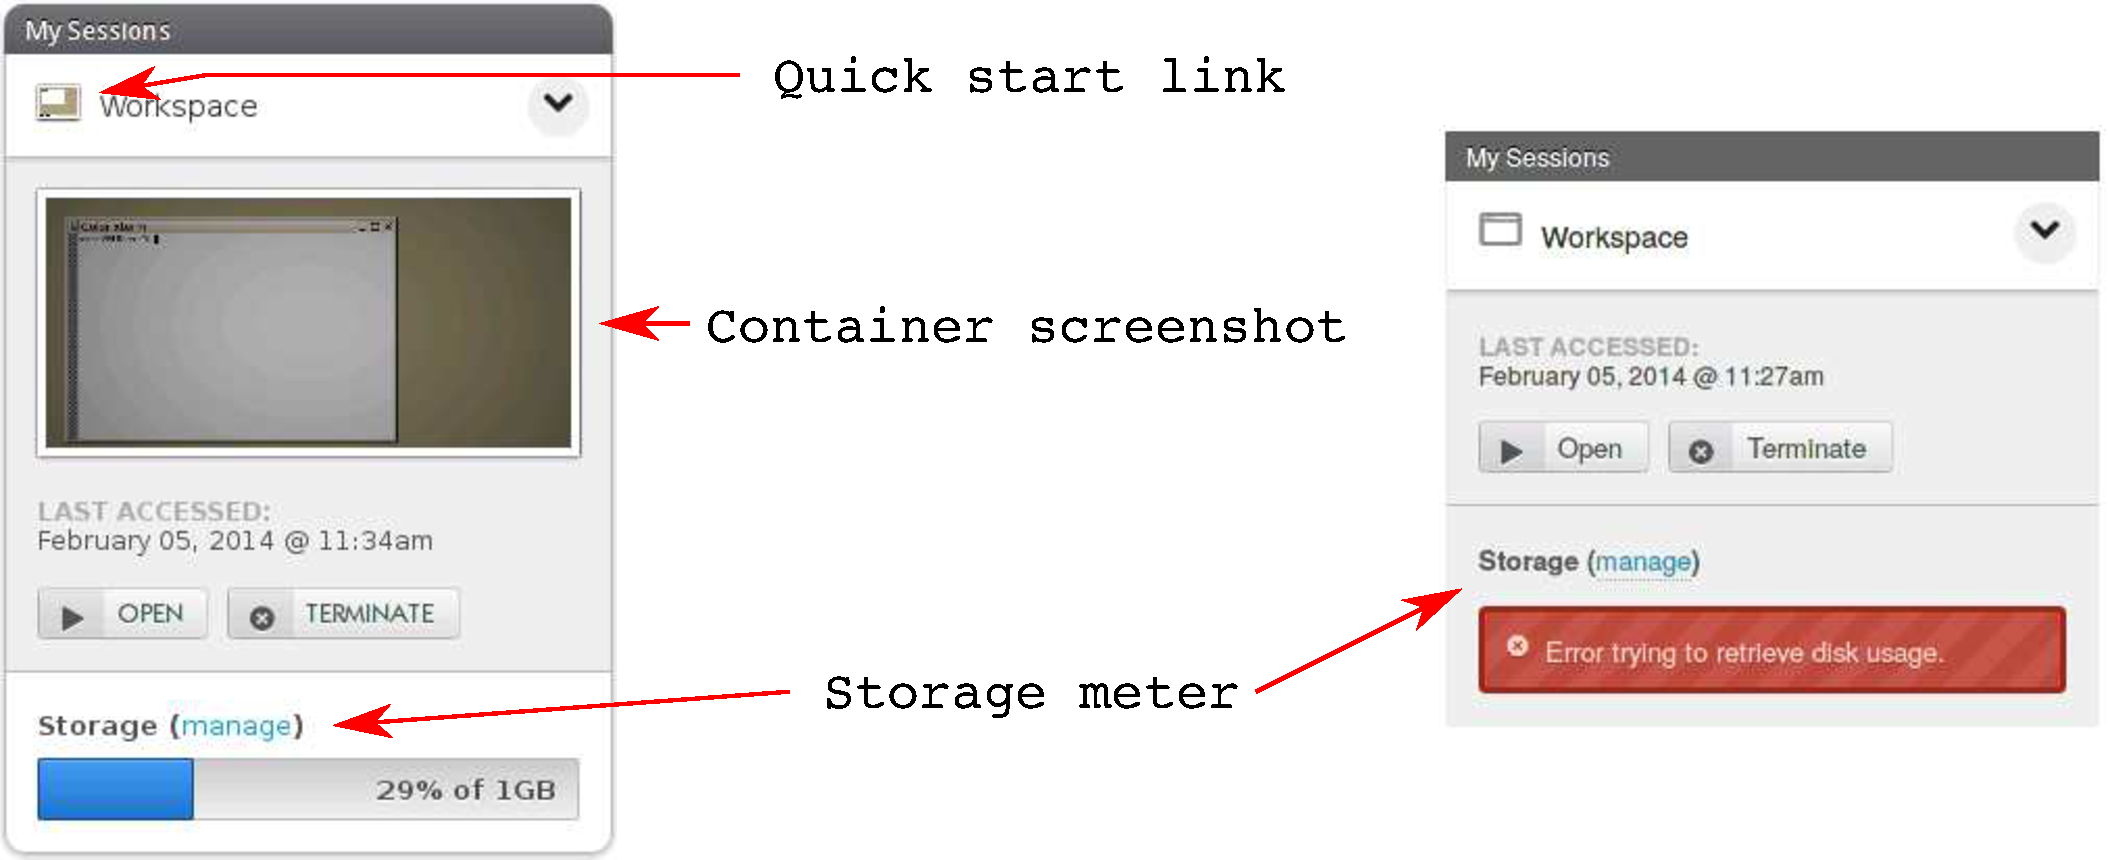
\includegraphics[width=\textwidth]
    {../../images/eps/hub+configuration+dashboard+my+sessions+2.pdf}
  \caption{ The \textit{My Sessions} module can be configured to show
            screen shots of the tool session containers, provide short
            cut links to access the container, and display the user's
            available disk store on the hub. The module on the left
            is fully configured showing the container screenshot, an
            enabled quick start link, and storage meter. The module
            on the right has some of these features disabled.}
  \label{fig:my_sessions_module_compare}
\end{figure}

The My Sessions module can be configured to provide the user with a shortcut
link to access active tool session containers and screen shots of applications
running inside of an active tool session container.  Capturing screen shots of
the tool session container is a function performed by the middleware and is not
available in the open source release, but hubs managed by the HUBzero group can
take advantage of this feature.

Similarly, the availability of the disk usage and quota information depends
upon the hub being configured to show the information and having the
\textit{telequotad}
% FIXME: should probably cite hubzero-telequotad
service running on the hub's fileserver. When the hub is not configured to show
the disk usage, or the telequotad service is not running, users are shown
messages like those in the image on the right side of Figure
\ref{fig:my_sessions_module_compare}, explaining that the information is
unavailable, or simply stating the used disk space is \textbf{0\% of 0GB} when
the user has no quota set.

When a hub is first installed, there are many settings that can be adjusted to
change the user experience. HUBcheck provides a library to help developers
automate the verification of these settings through the hub's website, from the
user's perspective. Using HUBcheck, developers can writing automation scripts,
that can login to the hub website as a user, start a tool session container,
and test if the My Sessions module is correctly showing screen shots and
enabling short cut links for the tool session container.


Developers can also write HUBcheck based automation scripts to identify
problems like the improper disk usage calculation mentioned earlier. To do this
by hand, a developer would:

\begin{figure}[H]
  \vspace{-10pt}
  \begin{minipage}[c]{0.48\linewidth}
    \begin{enumerate}
    \item login to the hub website as a user
    \item navigate to the user's Dashboard web page
    \item locate and read the disk storage string from the web page
    \item validate the string holds the proper format
    \end{enumerate}
  \end{minipage}
  \hfill
  \begin{minipage}[c]{0.48\linewidth}
    \centering
    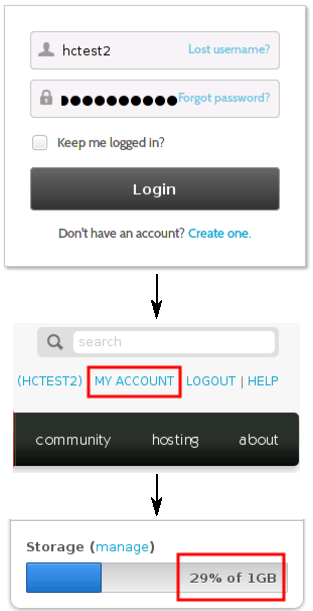
\includegraphics[scale=0.7]
      {../../images/eps/check+user+storage+meter+process+2.pdf}
%    \caption{Process to check that the user's storage meter is being displayed.}
    \caption{Accessing user's storage meter.}
    \label{fig:check_user_storage_meter_process}
  \end{minipage}
\end{figure}

\begin{xcode}{%
  language=Python,%
  label=fig:dashboard_mysessions_check_storage,%
  caption={Checking user's storage meter, using a HUBcheck backed script} %
}
...
# launch the browser and navigate to hub website
hc.browser.get('https://hubzero.org')

# login to the hub website as a user
hc.utils.account.login_as(username,userpass)

# navigate to the user's Dashboard web page
po = hc.catalog.load_pageobject('GenericPage')
po.header.goto_myaccount()

# locate and read the disk storage string from the web page
po = hc.catalog.load_pageobject('MembersDashboardPage')
storage_amount = po.modules.my_sessions.storage.storage_meter()

# validate the string holds the proper format
assert storage_amount != '', 'invalid storage amount returned'
assert storage_amount != '0% of 0GB', 'user quotas not activated'
...
\end{xcode}


A HUBcheck script, shown in Listing
\ref{fig:dashboard_mysessions_check_storage}, would follow the same steps.  The
format of the disk storage string should match the format \textbf{X\% of YGB},
where X is an integer, ranging from 0 to 100, describing the percentage of the
user's available disk that has been used, and Y is a positive integer
describing the amount of disk space available to the user, in gigabytes.

HUBcheck's web automation library simplifies common tasks like logging into the
hub website and navigating to web pages. The library also provides abstractions
of hub web pages, called page objects, so developers can reuse common blocks of
code and use a standard library for locating elements on the web page.


\subsection{Hub upgrade issues}

Errors also tend to arise on the hub after software upgrades.  These types of
errors can usually be traced back to configuration changes in upgraded hub
modules, the release of errant software, or pre-existing errors on the upgraded
hub that manifest themselves after the upgrade. Running HUBcheck after a hub
has been upgraded can help identify errors related to hub upgrades before the
user experiences them.

\begin{figure}[ht]
  \centering
  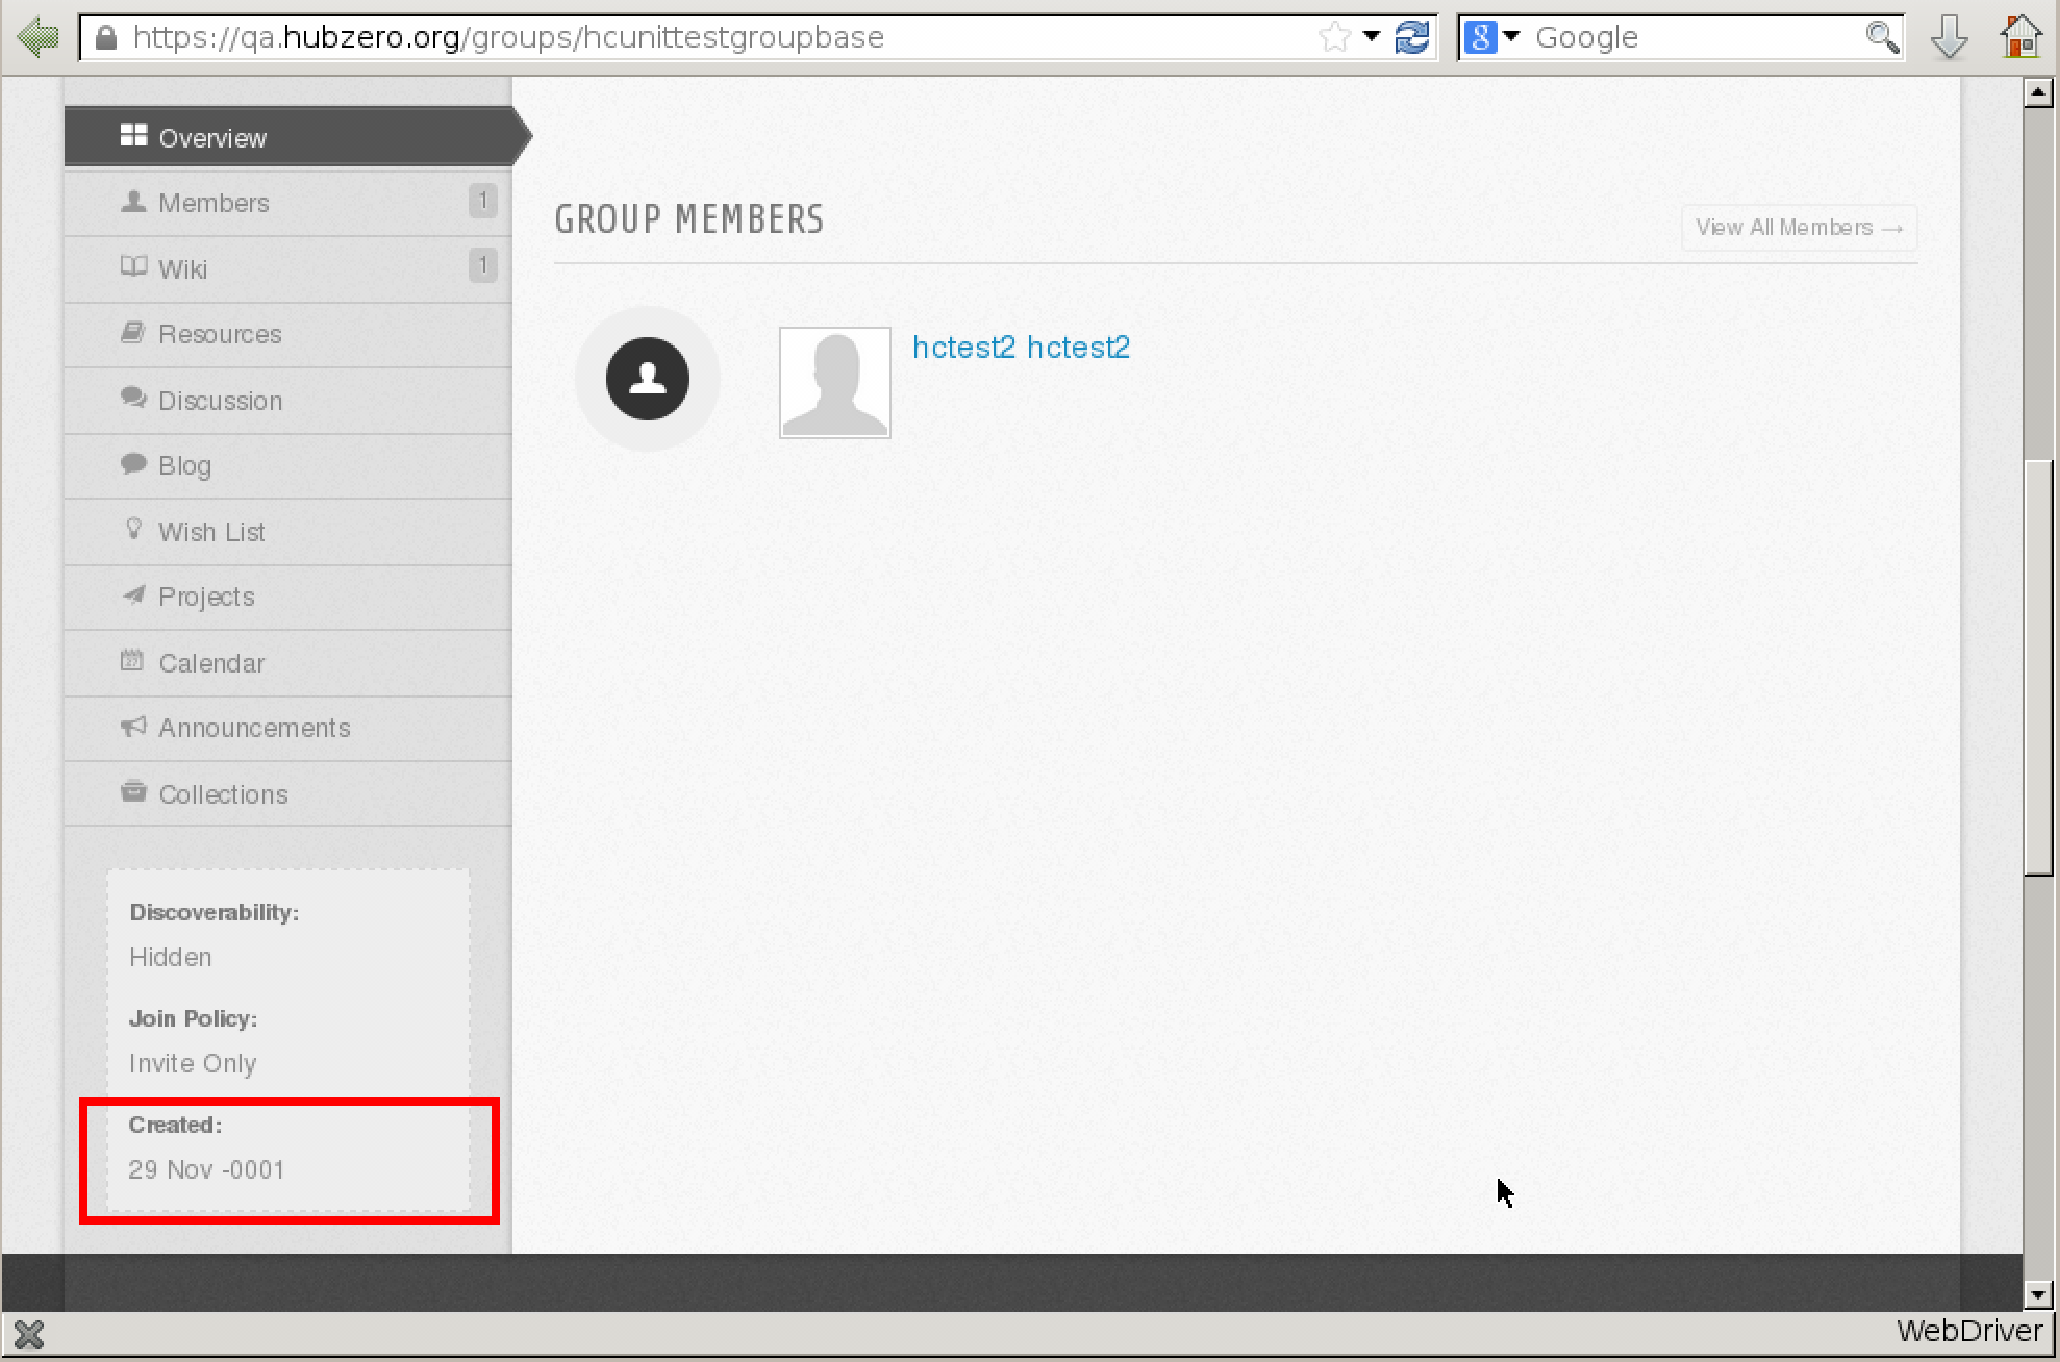
\includegraphics[width=0.5\textwidth]
    {../../images/eps/qahubzero_v1_2_group_create_date_bad_year.pdf}
  \caption{ Sometimes errors show up after a hub upgrade like this one, where
            the create date of a new hub group was not being displayed correctly.
            Finding this type of bug is tedious for a human, but developers
            can use HUBcheck to write tests and verify multistep processes,
            like creating a group, still produce expected results.}
  \label{fig:group_create_date_bad_year}
\end{figure}


One example of a hub upgrade related error HUBcheck was able to identify
occurred in the hub's \textit{Groups} component. The Groups component allows
users to organize content and discussions within the hub community. The
component provides discussion forums, wiki pages, blogs, project spaces and
more. Users can create a group by filling out a web form on the hub website.
Groups on the hub have an overview web page that provides some properties of the
group like group name, description, number of members, join policy and create
date.

After an upgrade of the Groups component was installed on a test hub as a part of
a hub software upgrade, HUBcheck was run, and developers were alerted to a
failing test.  The failing test was trying to verify the create date for a
newly created group on the hub. The HUBcheck test showed that the create date
of the group contained an invalid date. With knowledge of the problem, hub
developers were able to identify and fix the the errant code before it was was
propagated to more hubs, which would have resulted in additional cleanup work.

To find this type of error, a new group needed to be created on the hub, and
its properties validated. The process of creating a new group on the hub can be
tedious for a human, but with HUBcheck, it can be done in a few lines of code
in a testing script.


\subsection{Hub reboot issues}

When the servers hosting a hub are shut down and brought back up, it is easy
for unexpected problems to arise. From hosts having trouble rebooting to remote
filesystems not being properly mounted over the network, machine reboots are a
time where errors can happen that leave the hub not living up to its fullest
potential.  Developers can exercise hub functions quickly by running HUBcheck
after a reboot. HUBcheck provides the type of automation primitives that
encourage developers to tackle the harder problems to automate, like checking
that render servers are accepting connections from within a tool session
container.

\begin{figure}[ht]
  \centering
  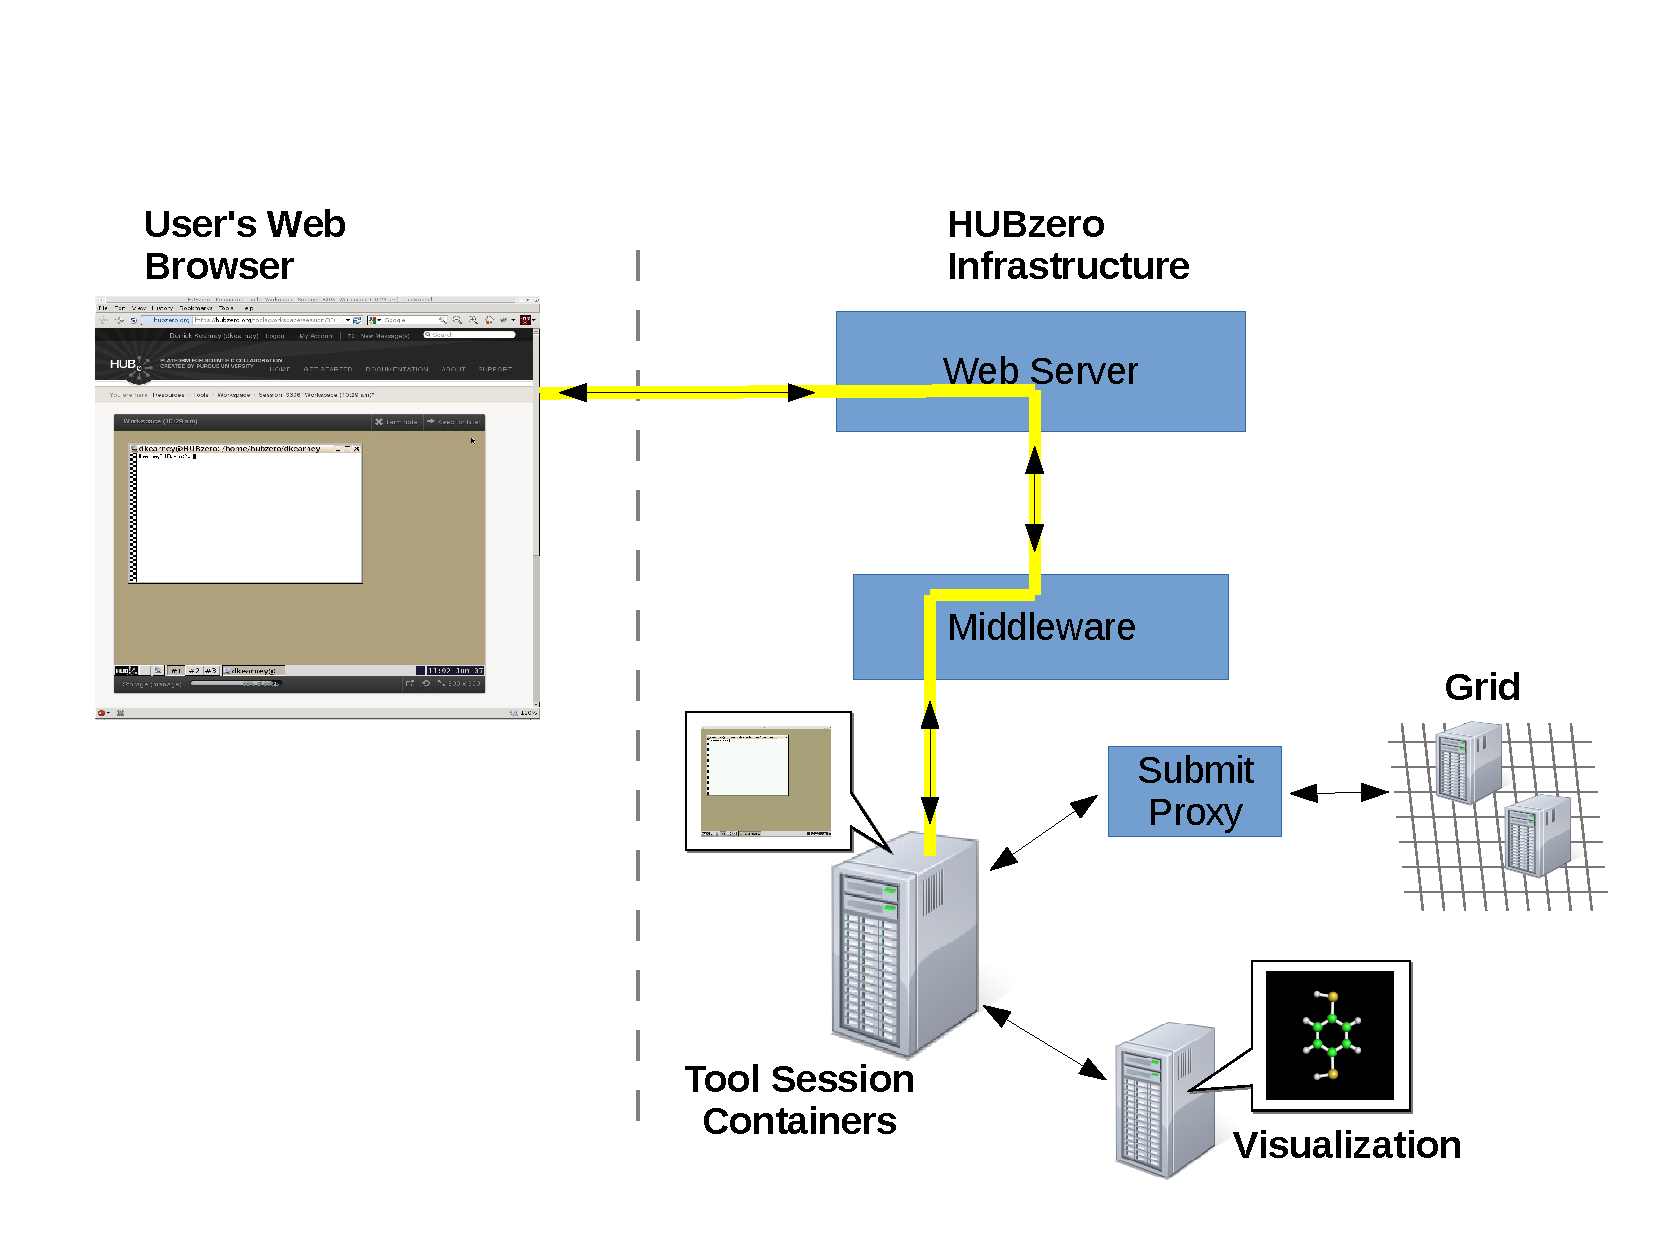
\includegraphics[width=\textwidth]
    {../../images/hubcheck_block_diagram/tool_session_container_block.pdf}
  \caption{ Simulation Tool developers use a tool session container to
            develop and deploy their work on the hub. }
  \label{fig:tool_session_container_block_diagram}
\end{figure}

One of the key features of a hub is its ability to run interactive simulation
tools that are displayed in the user's web browser. These simulation tools are
run in an environment called a tool session container, on an execution host
that is usually a part of the hub. In their web browser, the user sees a
display of the tool session container that has been projected to them, from the
hub, using the VNC protocol. Hosting the interactive simulation tools on the
hub allows them to take advantage of many features that would not normally be
found on the user's system, like access to grid computing services and powerful
rendering machines for interactive visualization.

The tool session container is a Debian Linux environment that supports the
building of simulation tools by tool developers and the execution of tools by
hub users. Access to grid computing and render machines are services provided
to the tool session containers. After a reboot of the hub these services should
be restored, and if they are not, the simulation tools may not work correctly.

There are two ways to access a tool session container. The most frequently used
way is through the web browser. Starting a tool on the hub gets the user access
to a tool session container. This approach doesn't allow the user to automate
interaction in a terminal with a shell. The second way is to connect over SSH,
the secure shell protocol. All tool developers can access a tool session
container in this way. This approach has the advantage that it gives access to
a terminal with a shell, and shell automation tools like Expect have existed
since the mid 1990s.

HUBcheck takes advantage of this second approach to accessing a tool session
container and provides a small, Expect like, shell automation library. Using
HUBcheck, developers can enter a tool session container and examine the
resources that are supposed to be available for tools to use, like access to
the render servers. Developers can write automated tests to check if a render
server is accepting connections from within the tool session container, under
the same conditions a simulation tool would be making its request from. This
type of access to the tool session container also allows developers to examine
container firewall setup, installation of software, like the \textit{Rappture
Toolkit}, access to grid infrastructures through the use of the \textit{submit}
command, file transfer between the user's desktop and the user's hub account
using the \textit{SFTP}, \textit{filexfer}, or \textit{webDAV} protocols, and
simulation tool invocation using \textit{invoke\_app}.


\section{Multimodal system automation}


HUBcheck's combination of web and shell automation libraries helps it provide
developers with the unique ability to write scripts that capture the user
experience of working in the dual environment system that is the hub. While a
great deal of testing and automation can be performed by libraries that only
access the website, or only access the tool session container, there exists a
set of tasks whose operations span both the website and the tool session
container, that no other single tool can automate. These are the cases of a
growing area of interest within the hub, where information is passed from
resources published on the website, to tools running inside of the tool session
container. In hub parlance, this is referred to as \textbf{parameter passing}.

Simulation tools run in a tool session container, either on the hub's web server
or on a separate execution host. While this approach has its advantages with
respect to deploying tools in a consistent environment, isolation between
different users running tools, and isolation between tools and the web server,
there are also a number of disadvantages, one of which is the inability to
easily pass parameters to the simulation tool before it has launched.

Launching a simulation tool on the hub involves coordination between both the
hub website and hub middleware. It can be explained in five steps:

\begin{enumerate}
\item User click's link to launch tool from web page.
\item Web link calls PHP function which forwards request to middleware.
\item Middleware starts a new tool session container for the tool.
\item Middleware calls tool's invoke script inside of the tool session container.
\item Invoke script execs command to start tool's graphical user interface.
\end{enumerate}

\begin{figure}[ht]
  \centering
  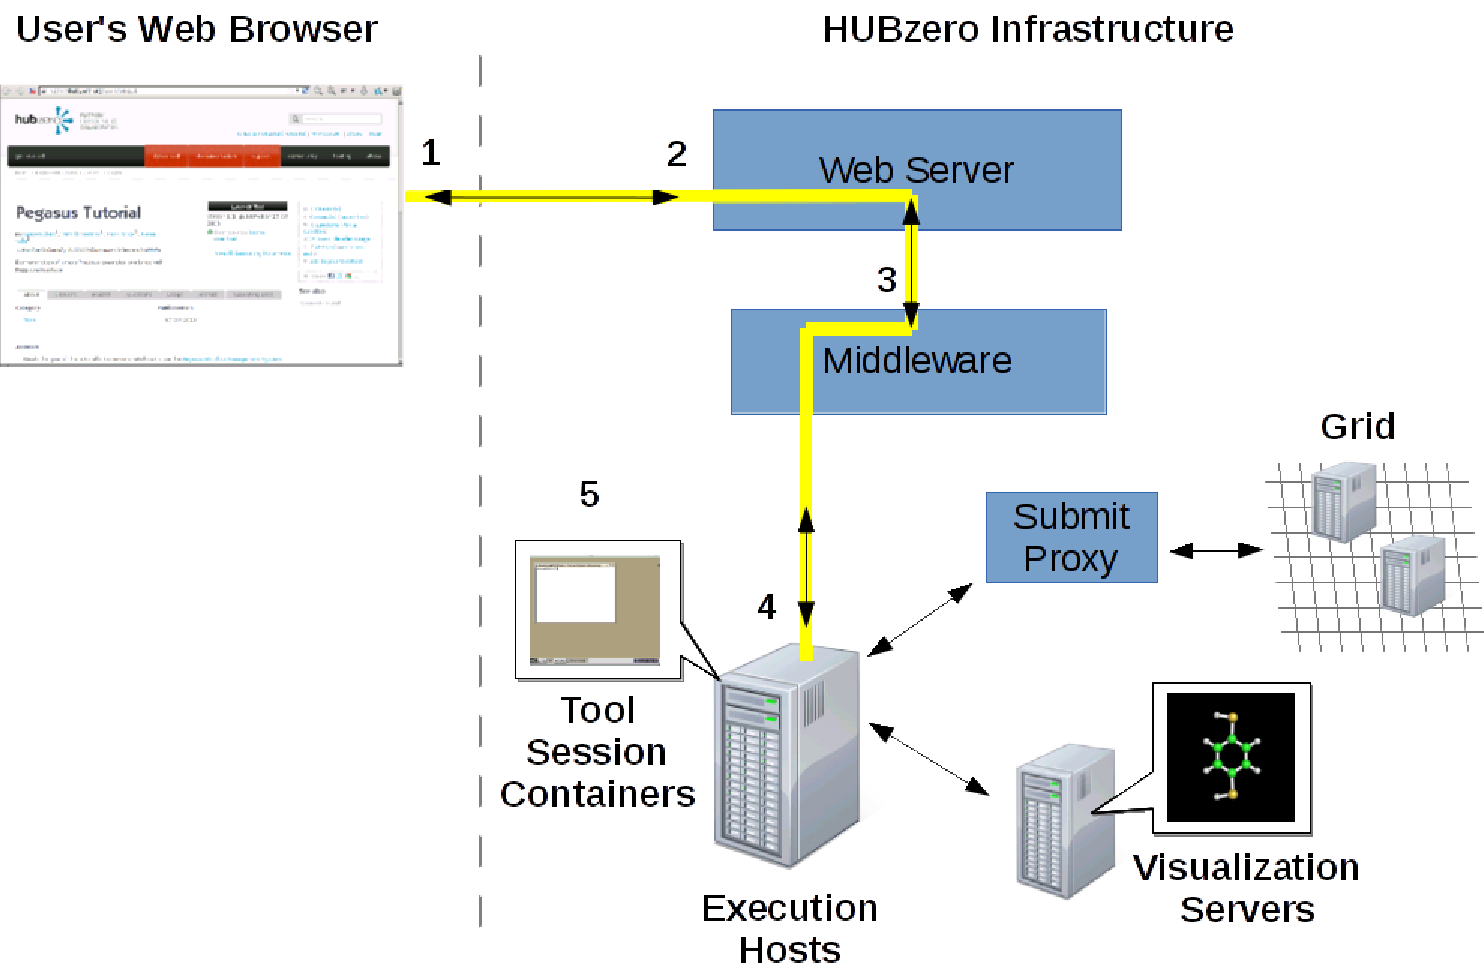
\includegraphics[width=\textwidth]
    {../../images/eps/start+tool+session+container+diagram2.pdf}
  \caption{ Simulation Tool are started by user's clicking a link on the hub
            website. The link forwards the request toe to the middleware, which
            handles allocating a tool session container and calling the tool's
            invoke script. The invoke script sets up the environment for the
            tool to run in, and finally, launches the tool.}
  \label{fig:start_tool_session_container_diagram}
\end{figure}

There are a couple of ways to start the process to launch a simulation tool on
the hub. The most apparent way is to use a web browser to navigate to the
tool's \textit{tool information page}. The tool information page is a web page
that describes what the tool does, the authors, other publications referencing
the tool, and how the development of the tool was funded. The tool information
page also includes a link to launch the tool. In the first step, the user
navigates to the tool information page and clicks the link to launch the tool.

% include a picture of a tool infomation page.

Clicking the web link sends a request to the hub web server asking it to start
the tool. The hub web server receives the request and calls upon the hub
middleware to launch the new tool.  In step three, the middleware starts a new
tool session container or dedicates a previously started tool session container
to run the requested tool.

Tools published on the hub include an \textit{invoke script} which contains all
of the commands necessary to launch the simulation tool, including setting up
system environment variables with prerequisite library and executable paths.
In step four above, the middleware enters the tool session container as the
user, and execs the tool's invoke script to start the graphical user interface.
Lastly, the invoke script sets environment variables for the libraries needed
by the tool and launches the tool.

Version 1.2 of the HUBzero software included new components that promote
allowing users to interact with learning concepts and data through the use of
simulation and modeling. Two examples of this include the Databases component
and the Courses component. The Databases component allows users to create
databases of information and construct views that help others understand their
data. The Courses component allows teachers to manage an online class, hosted
on the hub, that incorporates hub resources including simulation tools.  With
both of these components, developers may want pass data that is stored on the
hub website over to a tool running in a tool session container.

Version 1.2 of the HUBzero software also included a new algorithm for allowing
developers to pass parameters from the website into a simulation tool running
in a tool session container. The algorithm accepts a limited number of data
types (file names, directory names, and integers) and encodes the parameters
into the URL used to launch the tool. The parameters are passed through the hub
web server and middleware, which have the opportunity to check them for
validity, and into the tool session container. Once inside of the tool session
container, they are stored in a file, and the tool developer is responsible for
parsing them out of the file either through the tool's invoke script, or in the
simulation tool itself.

Whether it is data from a database being fed into a Cancer prediction model, or
example parameters for simulating a circuit from a class, passing data between
the website and the tool session container involves many layers of software
that have the opportunity to manipulate or lose the data. Passing data is
difficult to do and tedious to test.  HUBcheck provides the automation
primitives necessary to ease the task of writing scripts that can interact with
the website and tool session container, in the same script. In the case of
parameter passing, hub developers were able to use HUBcheck's web and shell
automation libraries to build a test suite to exercise passing parameters to a
simulation tool by crafting both valid and invalid URLs. As a part of the test
suite, numerous simulation tools were installed on the hub and URLs were
generated to match the requirements and restrictions of the parameter passing
algorithm. After launching tools with the specialized URLs, the HUBcheck based
scripts accessed the tool session container running the simulation tool, and
verified that the parameters were passed through the tool invocation labyrinth
that includes the web browser, the web server, the middleware, into the tool
session container, through the tool's invoke script, and to the tool where it
can be properly processed.


\end{document}
